\documentclass[14pt, aspectratio=169]{beamer}
\usetheme{Boadilla}
\usefonttheme{professionalfonts} % using non standard fonts for beamer
\usefonttheme{serif}
\usepackage{bm}
\usepackage{listings}
\usepackage{algorithm, algorithmic}
\usepackage{graphicx}
\usepackage{braket}
\usepackage{amsmath, amssymb, amsfonts}
\usepackage{url}
\usepackage[export]{adjustbox}
\usepackage{comment}

% \usepackage[backend=biber, style=authoryear]{biblatex}
% \addbibresource{references.bib}

% \usefonttheme[onlymath]{serif}


\setbeamertemplate{headline}{}
\setbeamertemplate{navigation symbols}{}
\setbeamercovered{transparent}
\setbeamertemplate{footline}[text line]{%
  \parbox{\linewidth}{\vspace*{-8pt} June 24 \hfill\hfill\insertpagenumber}}
\setcounter{tocdepth}{1}


\title{Course Scheduling Using Quantum Computing}
\author{\small{Mohammed Abdulsami \and Moustafa Salama \and Omar Abdelrasoul \\
\and Youssef AbdelWahab \and Yusuf Alsawah}}
\institute{UG Project \\ Supervised by: Dr. Ahmed ElMahdy, Dr. Marwa Sorour}

\date{June 2024}

\AtBeginSection[]
{
    \begin{frame}
        \frametitle{Table of Contents}
        \tableofcontents[currentsection]
    \end{frame}
}


\begin{document}

\maketitle

\begin{frame}{Table of Contents}
    \tableofcontents
\end{frame}

\section{Course scheduling problem}
\begin{frame}{Course Scheduling Problem}
    The course scheduling problem is about creating the best schedule for \textcolor{blue}{teachers} and \textcolor{blue}{classes} based on their available times slots.which makes it hard to find a good solution Because of its complexity.
\end{frame}

\begin{frame}{Problem Complexity}
    A Problem Complexity is categorized by the required time to solve it.\\[5mm]
    \textcolor{blue}{Complexity Classes}:\\
    \begin{itemize}
        \item \textit{P} class contains problems that can be solved in polynomial time
              \begin{itemize}
                  \item Array sorting is in \textit{P} class
                        %Recommended Change to: Sorting a list of numbers in ascending order
              \end{itemize}

        \item \textit{NP} class contains problems that can be solved in nondeterministic polynomial time
              \begin{itemize}
                  \item Time--Table scheduling problem is in \textit{NP} class
              \end{itemize}
    \end{itemize}
\end{frame}

\begin{frame}{Problem Complexity}

    The course scheduling problem is a \textcolor{blue}{combinatorial optimization problem}. This means we need to find the best schedule by minimizing the \textcolor{blue}{objective function}.
\end{frame}

\begin{frame}{Course Scheduling Problem}
    let us solve a simple course scheduling problem. For example, we have 2 Instructors and 2 classes also 2 available time slots. How we can present our problem?
\end{frame}

\begin{frame}{Course Scheduling Problem}
    \begin{figure}
        \centering
        \includegraphics[width=0.65\linewidth]{Table1.eps}
        \caption{Time Table}
        \label{fig:enter-label}
    \end{figure}
\end{frame}


\begin{frame}{Course Scheduling Problem}
    \begin{figure}
        \centering
        \includegraphics[width=0.65\linewidth]{Table2.eps}
        \caption{Instructor Available Time}
        \label{fig:enter-label}
    \end{figure}
\end{frame}

\begin{frame}{Course Scheduling Problem}
    \begin{figure}
        \centering
        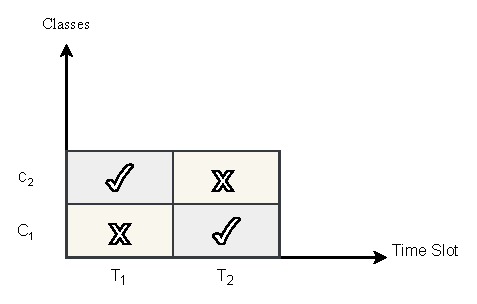
\includegraphics[width=0.65\linewidth]{Classes.eps}
        \caption{Classes Available Time}
        \label{fig:enter-label}
    \end{figure}
\end{frame}


% \section{Proposed Solution}

\section{Problem Formulation}

\begin{frame}{Problem Formulation}
    \begin{itemize}
        \item $N$: Number of instructors
        \item $M$: Number of classes
        \item $T$: is a set consisting of \(\{T_1, T_2, ...T_N\}\), where $T_i$ is a binary string containing the available hours for teaching for an instructor $i$.
        \item $C$: is a set consisting of \(\{C_1, C_2, ...C_M\}\), where $C_j$ is a binary string containing the available hours for studying for a class $j$.
        \item $R$: Matrix of \(M*N\) size where \(R_{ij}\) denotes the number of hours that instructor $i$ is required to teach class $j$
    \end{itemize}
\end{frame}

\begin{frame}{Problem Formulation}
    Our problem will be:
    \vspace{0.2cm}
    \begin{itemize}
        \item $N$: 2
        \item $M$: 2
        \item $T$: \{10 , 01\}
        \item $C$: \{10 , 01\}
        \item $R:
                  \begin{bmatrix}
                      1 & 0 \\
                      0 & 1
                  \end{bmatrix}$
    \end{itemize}
\end{frame}

\begin{frame}{Problem Formulation}
    \begin{itemize}
        \item $f(i,j,h) = 1 \xrightarrow{} h \in T_{i} \cap C_{j}$
              \vspace{2mm}
              \begin{itemize}
                  \item The function will yield 1 if both instructor $i$ and class $j$ are available in $h$ hour.
              \end{itemize}
              \vspace{2mm}

        \item \(\sum\limits_{h \in H} f(i,j,h) = R_{ij} \) , for all $1 \leq i \leq N$ and $1 \leq j \leq M$
              \vspace{2mm}
              \begin{itemize}
                  \item Assures that instructor $i$ teaches class $j$ the required number of hours during the week.
              \end{itemize}
              \vspace{2mm}
    \end{itemize}
\end{frame}
\begin{frame}{Problem Formulation}
    \begin{itemize}
        \item \( \sum\limits_{i=1}^{N} f(i,j,h) \leq 1 \) , for all $h \in H$ and $1 \leq j \leq M$
              \vspace{2mm}
              \begin{itemize}
                  \item Assures that each $j$ class does not have multiple instructors simultaneously.
              \end{itemize}
              \vspace{2mm}

        \item \( \sum\limits_{j=1}^{M} f(i,j,h) \leq 1 \) , for all $1 \leq i \leq N$ and $h \in H$
              \vspace{2mm}
              \begin{itemize}
                  \item Assures that each $i$ instructor does not teach multiple classes simultaneously.
              \end{itemize}
    \end{itemize}
\end{frame}

\section{QUBO Problem Formulation}

\begin{frame}{Quadratic Unconstrained Binary Optimization }
    To run the previous formulation on a quantum computer we need to convert the previous mathematical problem to Quadratic Unconstrained Binary Optimization (QUBO) problem.\\
\end{frame}

\begin{frame}{Quadratic Unconstrained Binary Optimization }
    QUBO stands for:
    \begin{itemize}
        \item Quadratic
              \begin{itemize}
                  \item Our equations are from the second degree (ie. $x^2$ or $x\cdot y$).
              \end{itemize}
              \vspace{2mm}
        \item Unconstrained
              \begin{itemize}
                  \item We will introduce slack terms to turn inequalities to equalities and do not forget to square it to avoid negative values.
              \end{itemize}
              \vspace{2mm}
        \item Binary
              \begin{itemize}
                  \item We use binary numbers only we can not use decimal numbers
              \end{itemize}
              \vspace{2mm}
        \item Optimization
              \begin{itemize}
                  \item We are trying to find the best solution either by minimizing or maximizing.
              \end{itemize}
    \end{itemize}
\end{frame}

\begin{frame}{QUBO Problem Formulation}
    \centering
    \begin{equation}
        \sum\limits_{h \in H} f(i,j,h) = R_{ij} \text{ , for all $1 \leq i \leq N$ and $1 \leq j \leq M$}
    \end{equation}
    \bigg\downarrow\\
    \begin{equation}
        \sum_{i=1}^{N} \sum_{j=1}^{M} \left(\sum_{h\in H} f(i,j,h) - R_{ij}\right)^2
        \label{qubo1}
    \end{equation}\\
    \vspace{0.2cm}
    Check that every instructor $i$ taught the required hours for class $j$ class
    \vspace{0.5cm}
\end{frame}

\begin{frame}{QUBO Problem Formulation}
    \centering
    \begin{equation}
        \sum\limits_{i=1}^{N} f(i,j,h) \leq 1 \text{ , for all $h \in H$ and $1 \leq j \leq M$}
    \end{equation}
    \bigg\downarrow\\
    \begin{equation}
        \sum\limits_{h \in H} \sum\limits_{j=1}^{M} \left(\sum\limits_{i=1}^{N} f(i,j,h)+\tau_{jh}-1\right)^2
    \end{equation}\\
    \vspace{0.2cm}
    Check that every $C_j$ class will be available at $h$ hour
    \vspace{0.5cm}
\end{frame}

\begin{frame}{QUBO Problem Formulation}
    \centering
    \begin{equation}
        \sum\limits_{j=1}^{M} f(i,j,h) \leq 1 \text{ , for all $1 \leq i \leq N$ and $h \in H$}
    \end{equation}
    \bigg\downarrow\\
    \begin{equation}
        \sum\limits_{h \in H} \sum\limits_{i=1}^{N} \left(\sum\limits_{j=1}^{M} f(i,j,h)+\lambda_{ih}-1\right)^2
    \end{equation}\\
    \vspace{0.2cm}
    Check that every $T_i$ teacher will be available at $h$ hour
    \vspace{0.5cm}
\end{frame}

\begin{frame}{QUBO Formulation}
    \centering
    \begin{equation}
        \begin{split}
            \min\sum\limits_{h \in H} \sum\limits_{i=1}^{N} \left(\sum\limits_{j=1}^{M} f(i,j,h)+\lambda_{ih}-1\right)^2 + \\
            \sum\limits_{h \in H} \sum\limits_{j=1}^{M} \left(\sum\limits_{i=1}^{N} f(i,j,h)+\tau_{jh}-1\right)^2 + \\
            \sum_{i=1}^{N} \sum_{j=1}^{M} \left(\sum_{h\in H} f(i,j,h) - R_{ij}\right)^2 \\
        \end{split}
    \end{equation}
\end{frame}

\section{Quantum Computers}
\begin{frame}{Quantum Computing Types}
    There are two main types of Quantum Computers:\\
    \begin{itemize}
        \item Adiabatic Quantum Computer
        \item Gate-based Quantum Computer
    \end{itemize}
\end{frame}

\begin{frame}{Adiabatic Quantum Computer}
    Adiabatic Quantum Computer works based on the quantum adiabatic theorem:
    \begin{theorem}
        If a quantum system starts in a ground state, so long as we evolve the state slowly, it is likely to remain in a ground state.
    \end{theorem}
\end{frame}

\section{Hamiltonian}
\begin{frame}{Ground-state}
    The ground state of a quantum-mechanical system is its stationary state of lowest energy; the energy of the ground state is known as the zero-point energy of the system.
\end{frame}

\begin{frame}{Ground-state}
    \begin{figure}
        \centering
        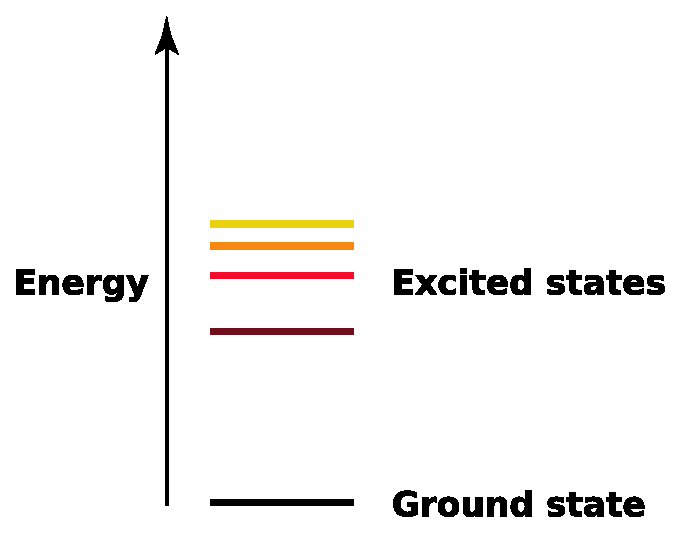
\includegraphics[width=0.4\linewidth]{images/illustration/Energy_levels.eps}
        \caption{Energy Levels}
        \label{fig:energy-levels}
    \end{figure}
\end{frame}

\begin{frame}{Wave Function}
    \begin{figure}
        \centering
        \includegraphics[width=\linewidth]{wave_ahmed.png}
        \caption{Caption}
        \label{fig:enter-label}
    \end{figure}
\end{frame}

\begin{frame}{Wave Function}
    If we have a plane and a wave traveling through the plane.
    When observing point $a$ and $b$ at anytime:
    \begin{figure}
        \centering
        \includegraphics[width=0.8\linewidth]{images/illustration/Wave.eps}
        \caption{Normal Plane}
        \label{fig:enter-label}
    \end{figure}
\end{frame}

\begin{frame}{Wave Function}
    What if the wave was time-independent? This is the stationary wave. It changes depending on the space, not the time.
    \begin{figure}
        \centering
        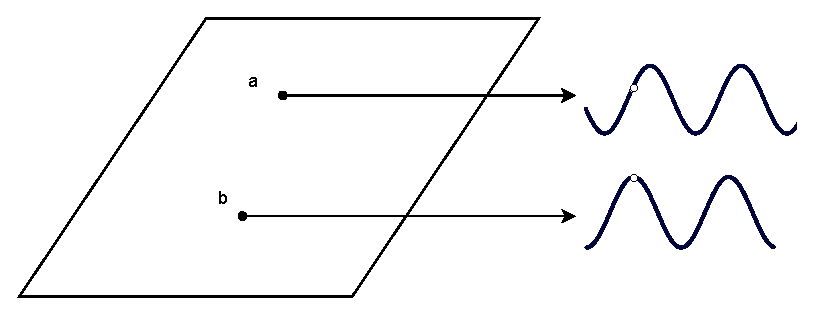
\includegraphics[width=0.8\linewidth]{NewWave.eps}
        \caption{Stationary Wave Plane}
        \label{fig:enter-label}
    \end{figure}
\end{frame}

\begin{frame}{Hamiltonian}
    Simply, the Schrödinger equation is based on Hamiltonian.
    % \[i\hbar \frac{\partial}{\partial t} \ket{\Psi(t)} = \hat H \ket{\Psi(t)}\]
    \[\ket{\Psi_{t}} = e^{-iHt}\ket{\Psi_{0}}\]
    Hamiltonian is an operator that describes the KE and PE of a system. It operates
    on the input state and is a key operator in the Schrödinger equation.
\end{frame}


\begin{frame}{Schrödinger Equation}
    Time-independent equation:
    \[H\ket{x} = f(x)\ket{x}\]
    By solving this equation we get eigenstates. Eigenstates are subsets of possible classical output and they are stationary waves. As we can see the state does not change because this equation is time dependent. Also by solving f eigenvectors that have the smallest eigenvalue.
\end{frame}

\begin{frame}{Schrödinger Equation}
    Time-dependent equation:
    \[\ket{\Psi_{t}} = e^{-iHt}\ket{\Psi_{0}}\]
    \begin{itemize}
        \item $\ket{\Psi_{t}}$ is the state at $t$ time.
        \item $i$ is the imaginary number.
        \item $t$ is the time.
        \item $\hat H$ is the Hamiltonian.
    \end{itemize}
\end{frame}

\begin{frame}{Schrödinger Equation}
    Time-dependent equation:
    \[\ket{\Psi_{t}} = e^{-iHt}\ket{\Psi_{0}}\]
    This equation evolves the state over time, unlike the previous equation.
    We use the following table to convert terms to the corresponding Hamiltonian.
\end{frame}


\begin{frame}{Hamiltonian}
    \begin{table}[ht]
        \label{tab:Table1}
        \centering
        \begin{tabular}{||c | c ||}
            \hline
            \(f(x)\)               & \(H_f\)                                            \\[2mm]
            \hline
            \hline
            \({x}\)                & $\frac{1}{2}I - \frac{1}{2}Z$                      \\[2mm] \hline\(\overline{x}\)& $\frac{1}{2}I - \frac{1}{2}Z$\\[2mm]
            \hline
            \({x}_1 \oplus {x}_2\) & $\frac{1}{2}I - \frac{1}{2}Z$                      \\[2mm]
            \hline
            \({x}_1 \land{x}_2\)   & \(\frac{1}{4}I - \frac{1}{4}(Z_1 + Z_2 - Z_1Z_2)\) \\[2mm] \hline
        \end{tabular}
        \caption{Hamiltonians Representing Basic Boolean Clauses}
    \end{table}
\end{frame}

\begin{frame}{Adiabatic theorem}
    Adiabatic theorem:
    \begin{itemize}
        \item We start with initial Hamiltonian, {\color{blue} $H_{i}$}, whose ground-state
              is easy to prepare
              % \begin{itemize}
              %   \item Easy to prepare means that you can create it easily.
              % \end{itemize}
        \item We evolve our {\color{blue} $H_{i}$} slowly until we reach the {\color{blue}
                      $H_{f}$}
        \item The final Hamiltonian, {\color{blue} $H_{f}$}, whose ground-state is the
              solution for our problem.
              % \item 
    \end{itemize}
\end{frame}

\section{QAOA Problem Formulation}

\begin{frame}{Quantum Approximate Optimization Algorithm}
    Quantum Approximate Optimization Algorithm (QAOA) relies on trotterization to find approximate solutions.
    Our Hamiltonian:
    \[H = H_{i} + H_{p}\]
    \begin{itemize}
        \item $H_{i}$: Initial Hamiltonian
        \item $H_{p}$: Problem Hamiltonian
    \end{itemize}
\end{frame}

\begin{frame}{Quantum Approximate Optimization Algorithm}
    \begin{figure}
        \centering
        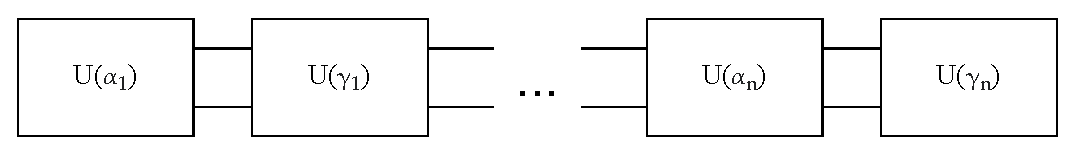
\includegraphics[width=\linewidth]{images/illustration/QAOA.eps}
        \caption{Trotterization}
        \label{fig:enter-label}
    \end{figure}
\end{frame}

\begin{frame}{Quantum Approximate Optimization Algorithm}
    \begin{figure}
        \centering
        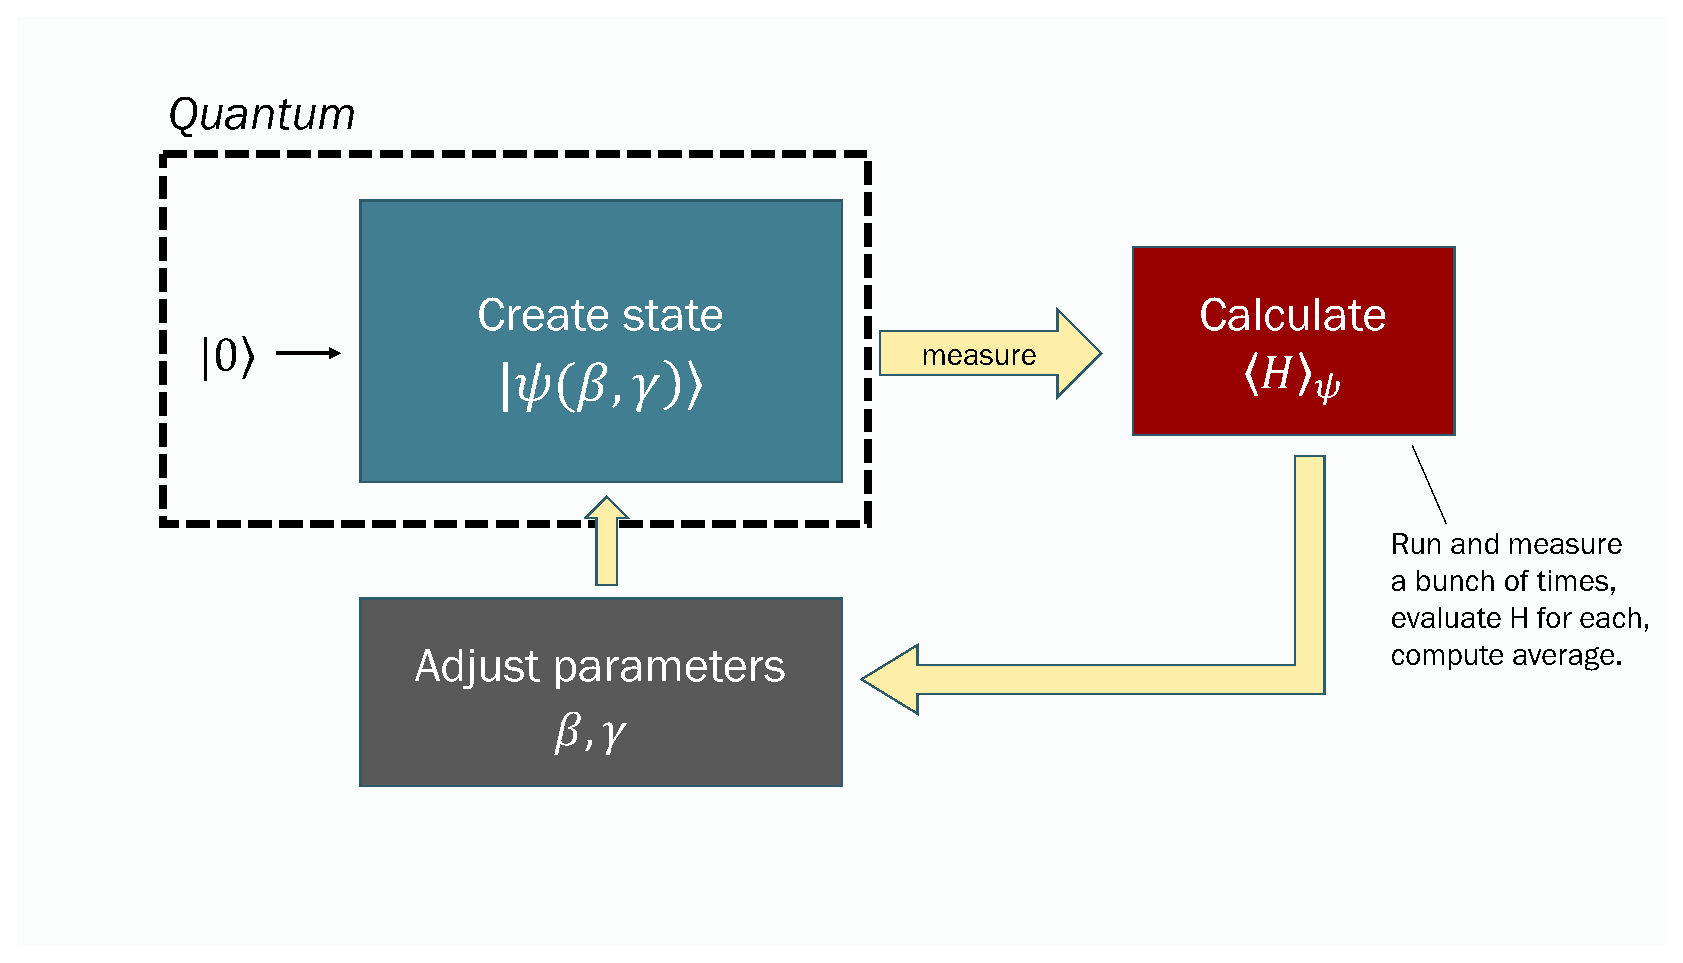
\includegraphics[width=0.75\linewidth]{qaoa_System_Slide.eps}
        \caption{QAOA Overview (NC State University)}
        \label{fig:enter-label}
    \end{figure}
    \footnote{ECE 592/CSC 591, NC State University, Fall 19}
\end{frame}
\begin{comment}
\begin{frame}{QAOA}

    \centering {\textcolor{blue}{Quantum Approximate Optimization Algorithm}}\\

    % \begin{comment}
    \vspace{2mm}
    How it work:\hfill
    \vspace{2mm}
    \begin{itemize}
        \item Initialization
              \begin{itemize}
                  \item We prepare the initial state. For example, put all qubits in superposition.
              \end{itemize}
        \item Problem Hamiltonian
              \begin{itemize}
                  \item We convert the problem Hamiltonian to the corresponding quantum gates.
              \end{itemize}
        \item Mixing Hamiltonian
              \begin{itemize}
                  \item We convert the mixing Hamiltonian to the corresponding quantum gates to explore possible solutions.
              \end{itemize}
        \item Classical optimizer
              \begin{itemize}
                  \item After computing the expectation by measuring the circuit we use a classical optimizer to find optimal parameters
              \end{itemize}

    \end{itemize}
    % \end{comment}
\end{frame}
\end{comment}
\begin{frame}{Hamiltonian construction}
    Conversion steps:
    \begin{itemize}
        \item We expand an equation
        \item We select the appropriate role from the table
        \item We raise this role to $e^{-iH}$
        \item Simplify the equation
        \item Finally find corresponding gates.
    \end{itemize}
\end{frame}

\begin{frame}{Hamiltonian construction}
    Let's expand equation \ref{qubo1}:
    \vspace{2mm}
    \[\sum_{i=1}^{2} \sum_{j=1}^{2} \left(\sum_{h\in H} f(i,j,h) - R_{ij}\right)^2 \]

\end{frame}

\begin{frame}{Hamiltonian construction}
    $f$ equation after expansion:\\
    \[f(1,1,1)^{2} + 2 f(1,1,1) f(1,1,2) - 2 f(1,1,1) + f(1,1,2)^{2} + ...\]
    \begin{itemize}
        \item 1 is a trivial term
        \item other terms are non-trivial terms
    \end{itemize}
    \vspace{4mm}
    When we convert trivial they result in an identity matrix that does not affect the output so it is better to discard them.
\end{frame}


\begin{frame}{Hamiltonian construction}
    Let's take $-2f(1,1,1)$:
    \begin{itemize}
        \item Coefficient: -2
        \item Used role: \({x}\) = $\frac{1}{2}I - \frac{1}{2}Z$
    \end{itemize}
    \vspace{2mm}
    Conversion:
    \[-2f(1,1,1) \rightarrow \frac{1}{2}I - \frac{-2}{2}Z \rightarrow \frac{1}{2}I + Z \rightarrow Z\]
\end{frame}

\begin{frame}{Hamiltonian conversion}
    Let's take $-2f(1,1,1)$:
    \begin{itemize}
        \item Coefficient: -2
        \item Used role: \({x}\) = $\frac{1}{2}I - \frac{1}{2}Z$
        \item Rz($\lambda$) gate: $e^{-i\frac{\lambda}{2}Z}$
    \end{itemize}
    \vspace{2mm}
    Conversion:
    \[Z \rightarrow e^{-iZ} \rightarrow Rz(-2)\]
\end{frame}
%replace it%
\begin{frame}{Generated circuit}
    \begin{figure}
        \centering
        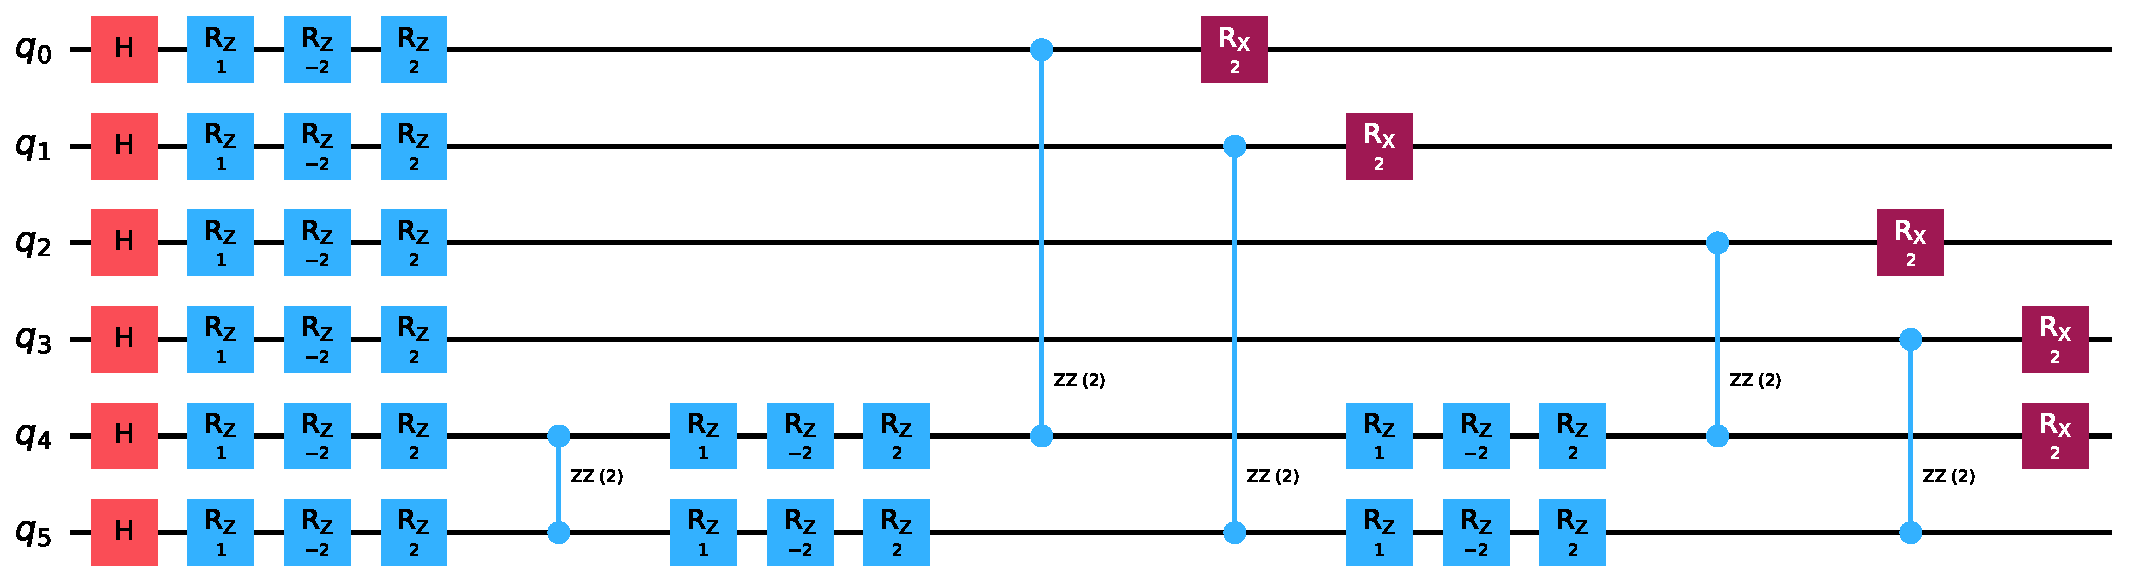
\includegraphics[width=1\textwidth]{images/illustration/6_qubit_circuit.eps}
        \caption{Simple circuit}
        \label{fig:6_qubit_circuit}
    \end{figure}
\end{frame}

\section{System Overview}
\begin{frame}{System Overview}
    \begin{figure}
        \centering
        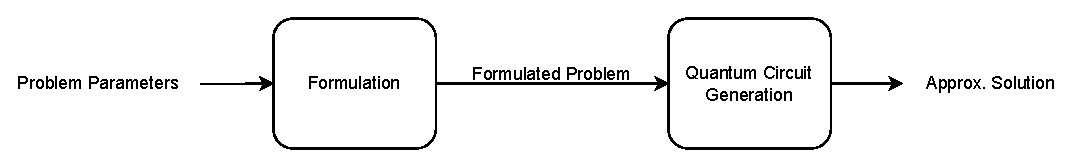
\includegraphics[width=\linewidth]{images/Diagram/SystemOverview.eps}
        \caption{System Overview}
        \label{fig:system_overview}
    \end{figure}
\end{frame}

\begin{frame}{System Overview}
    \begin{figure}
        \centering
        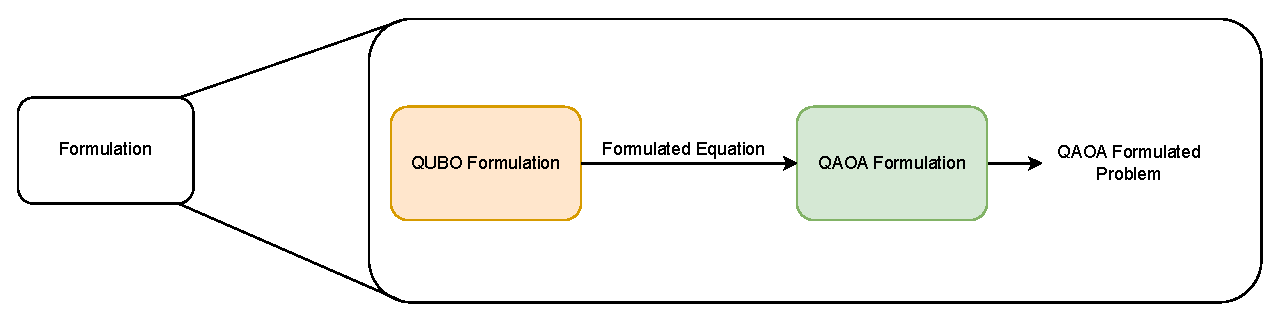
\includegraphics[width=\linewidth]{images/Diagram/Formulation.eps}
        \caption{Formulation Component}
        \label{fig:formulation}
    \end{figure}
\end{frame}

\begin{frame}{System Overview}
    \begin{figure}
        \centering
        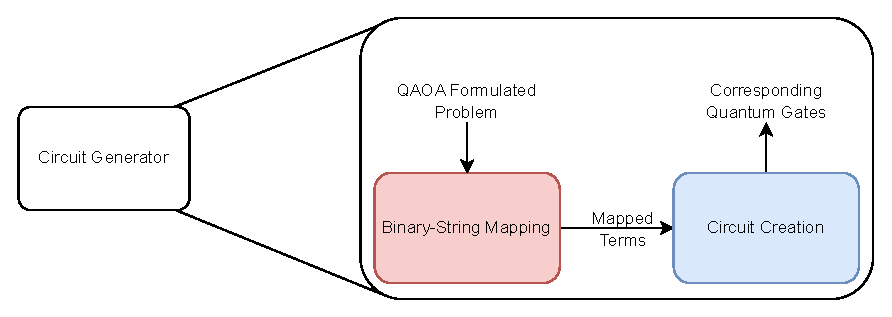
\includegraphics[width=\linewidth]{images/Diagram/CircuitGenerator.eps}
        \caption{Circuit Generator Copmponet}
        \label{fig:circiut_generator}
    \end{figure}
\end{frame}

\begin{frame}{Hamiltonian conversion}
    In the previous slide, we discussed how we map variables to the corresponding quantum gate.
    It is a straightforward process but it becomes infeasible with a large number of terms.\\
    \vspace{2mm}
    For Example:\\
    \begin{itemize}
        \item 3 Qubits will result in 15 terms.
        \item 6 Qubits will result in 30 terms.
        \item 175 Qubits will result in 1925 terms.
        \item 1440 Qubits will result in 27820 terms.
    \end{itemize}
\end{frame}

\begin{frame}{Hamiltonian conversion}
    The number of terms to be converted to Quantum gate increases rapidly, so converting them manually would be an error-prone solution in addition to its inconvenience.\\
\end{frame}

\begin{frame}{Circuit generator}
    As a solution, we created a simple circuit generator that facilitates the conversion process.\\
\end{frame}

\begin{frame}{Circuit generator}
    \begin{itemize}
        \item Takes the circuit configuration as a JSON file.
        \item Parses the input file.
        \item Output the result circuit.
    \end{itemize}
\end{frame}

\section{Results}

\begin{frame}{Experiment configuration}
    These are the used configurations to produce these results.\\
    \begin{itemize}
        \item Random seed = 10
        \item Shots = 10240
        \item p-layers = 5
    \end{itemize}
\end{frame}

\begin{frame}{Result decoding}
    When we run a quantum circuit it outputs the result as a bit-string it may be gibberish until you understand it.\\
\end{frame}

\begin{frame}{Result decoding}
    \begin{figure}
        \centering
        % it is png :)
        \includegraphics[width=0.40\linewidth]{images/illustration/16_qubit_hitsto.png}
        \caption{16-qubit circuit results}
        \label{fig:16_qubit_result}
    \end{figure}
\end{frame}

\begin{frame}{Result decoding}
    \begin{figure}
        \centering
        \includegraphics[width=0.7\linewidth]{images/illustration/bin_string_1.eps}
        \caption{Bit-string}
        \label{fig:bin_string_1}
    \end{figure}
\end{frame}

\begin{frame}{Result decoding}
    \begin{figure}
        \centering
        \includegraphics[width=0.7\linewidth]{images/illustration/bin_string_2.eps}
        \caption{Bit-string}
        \label{fig:bin_string_2}
    \end{figure}
\end{frame}

\begin{frame}{Result decoding}
    \begin{figure}
        \centering
        \includegraphics[width=0.7\linewidth]{images/illustration/bin_string_3.eps}
        \caption{Bit-string}
        \label{fig:bin_string_3}
    \end{figure}
\end{frame}

\begin{frame}{Result}
    \begin{figure}
        \includegraphics[width=0.55\linewidth]{images/prob_solutions/16_5_10240_prob-solution.eps}
        \caption{16-Qubit Solution Distribution  }
        \label{fig:cost_prob_16}
    \end{figure}
\end{frame}

\begin{frame}{Result}
    \begin{figure}
        \includegraphics[width=0.5\linewidth]{images/p_iterations/16_all_p-iteration.eps}
        \caption{Effect of changing the no of layers on the no of minimization steps for 16Q}
        \label{fig:cost_prob_6}
    \end{figure}
\end{frame}


\begin{frame}{Result}
    \begin{figure}
        \includegraphics[width=0.5\linewidth]{images/shots_solutions/16_all_shots-solution.eps}
        \caption{16-Qubit No. Shots and Solution Probability }
        \label{fig:cost_prob_24}
    \end{figure}
\end{frame}

\begin{frame}{Result}
    \begin{figure}
        \includegraphics[width=0.5\linewidth]{images/p_solutions/16_all_p-solution.eps}
        \caption{16-Qubit No. p-layers and Solution Probability }
        \label{fig:cost_prob_24}
    \end{figure}
\end{frame}

\begin{frame}{Current Work}
    \begin{itemize}
        \item Currently, experimenting with the formulation of the Flexible Open Shop Scheduling Problem to see if it produces better results.
        \item Waiting for feedback on our paper ``On the Practicality of Restricted Time-Table Problem Solution Using Quantum Approximate", which was submitted to IEEE Quantum Week. The results should return by the $15^{th}$ of July.
    \end{itemize}
\end{frame}

\begin{frame}{Future Work}
    \begin{itemize}
        \item Better initialize the problem variables to make the classical optimizer less time-consuming.
        \item Investigate grouping, to minimize/optimize the number of qubits needed for the circuit.
        \item Revisit the mathematical formulation of our Hamiltonians.
        \item Running more simulations on real Quantum Computers
    \end{itemize}
\end{frame}

\title{Thank you!}
\date{}
\author{}
\institute{}
\maketitle


\begin{frame}[allowframebreaks, noframenumbering]{References}
    \begin{thebibliography}{99}
        \bibitem{cambridge}
        D. Reppy, "Quantum Computing Lecture Notes," University of Cambridge, [Online]. Available: \url{https://www.cl.cam.ac.uk/teaching/2223/QuantComp/materials.html}. [Accessed: Jun. 3, 2024].

        \bibitem{ibm-learning}
        IBM, "IBM Quantum Experience," IBM, [Online]. Available: \url{https://learning.quantum.ibm.com/}. [Accessed: Jun. 3, 2024].

        \bibitem{qiskit}
        IBM, "Qiskit: An open-source quantum computing software development framework," IBM, [Online]. Available: \url{https://www.ibm.com/quantum/qiskit}. [Accessed: Jun. 3, 2024].

        \bibitem{Hamiltonians}
        S. Hadfield, ‘On the Representation of Boolean and Real Functions as Hamiltonians for Quantum Computing’, ACM Transactions on Quantum Computing, vol. 2, no. 4, p. 3, Dec. 2021.

        \bibitem{Lecture}
        QAOA Combinatorial Optimization, ECE 592/CSC 591, NC State University, Fall 2019
    \end{thebibliography}
\end{frame}




\end{document}

